\documentclass[0-protokol.tex]{subfiles}
\begin{document}

Tabulky \ref{tab:u1_1000} a \ref{tab:u1_inf} obsahují hodnoty vstupní charakteristiky tranzistoru. Pro měření v bázovém obvodu byly použity dva multimetry \textbf{METEX MXD-4660A}. Chyby hodnot byly určeny chybami těchto přístrojů. Nekonečný odpor byl realizován rozpojením kolektorového obvodu.
\begin{table}[H] 
\centering
\setlength{\tabcolsep}{10pt}
\begin{minipage}[t]{0.48\textwidth}
\begin{tabular}[t]{
    S[table-format=0.5]
    S[table-format=0.5]
    S[table-format=2.3]
    S[table-format=0.3]
} \toprule
{$U_{BE}$}   & {$\sigma_{U_{BE}}$} & {$I_{BE}$}    & {$\sigma_{I_{BE}}$} \\
{$[\si{V}]$} & {$[\si{V}]$}        & {$[\si{mA}]$} & {$[\si{mA}]$}       \\ \midrule
0.54380      & 0.00003             & 0.001         & 0.003               \\
0.58570      & 0.00003             & 0.004         & 0.003               \\
0.61610      & 0.00004             & 0.082         & 0.003               \\
0.63100      & 0.00004             & 0.222         & 0.003               \\
0.66460      & 0.00004             & 0.818         & 0.003               \\
0.68290      & 0.00004             & 1.474         & 0.003               \\
0.69140      & 0.00004             & 1.922         & 0.004               \\
0.70580      & 0.00004             & 2.989         & 0.004               \\
0.71570      & 0.00004             & 4.039         & 0.005               \\
0.73110      & 0.00004             & 6.400         & 0.006               \\
0.74620      & 0.00004             & 9.987         & 0.008               \\
0.76420      & 0.00004             & 16.57         & 0.02                \\
0.78090      & 0.00004             & 25.64         & 0.02                \\
0.78820      & 0.00004             & 30.69         & 0.02                \\
0.79950      & 0.00004             & 39.84         & 0.03                \\ \bottomrule
\end{tabular}
\caption{Naměřené hodnoty napětí a proudu v bázovém obvodu zapojení \ref{fig:zap_u12} při odporu $R_2 = \SI{1000}{\ohm}$}
\label{tab:u1_1000}
\end{minipage}
\hfill
\begin{minipage}[t]{0.48\textwidth}
\begin{tabular}[t]{
    S[table-format=0.5]
    S[table-format=0.5]
    S[table-format=2.3]
    S[table-format=0.3]
} \toprule
{$U_{BE}$}   & {$\sigma_{U_{BE}}$} & {$I_{BE}$}    & {$\sigma_{I_{BE}}$} \\
{$[\si{V}]$} & {$[\si{V}]$}        & {$[\si{mA}]$} & {$[\si{mA}]$}       \\ \midrule
0.37660      & 0.00002             & 0.000         & 0.003               \\
0.50270      & 0.00003             & 0.043         & 0.003               \\
0.55900      & 0.00003             & 0.033         & 0.003               \\
0.60860      & 0.00004             & 0.169         & 0.003               \\
0.61990      & 0.00004             & 0.241         & 0.003               \\
0.64220      & 0.00004             & 0.472         & 0.003               \\
0.66200      & 0.00004             & 0.851         & 0.003               \\
0.67890      & 0.00004             & 1.404         & 0.003               \\
0.68970      & 0.00004             & 1.933         & 0.004               \\
0.71610      & 0.00004             & 4.234         & 0.005               \\
0.73030      & 0.00004             & 6.435         & 0.006               \\
0.74410      & 0.00004             & 9.600         & 0.008               \\
0.75790      & 0.00004             & 14.15         & 0.01                \\
0.76920      & 0.00004             & 19.20         & 0.02                \\
0.78420      & 0.00004             & 28.12         & 0.02                \\
0.79270      & 0.00004             & 34.47         & 0.02                \\
0.80050      & 0.00004             & 41.18         & 0.03                \\ \bottomrule
\end{tabular}

\caption{Naměřené hodnoty napětí a proudu v bázovém obvodu zapojení \ref{fig:zap_u12} při odporu $R_2 = \inf$}
\label{tab:u1_inf}
\end{minipage}
\end{table}

V tabulkách \ref{tab:u2_0.1}, \ref{tab:u2_0.2} a \ref{tab:u2_0.3} jsou zaznamenány hodnoty naměřené v rámci úkolu 2, tedy výstupní charakteristiky tranzistoru. Měření bylo v kolektorovém obvodu provedeno multimetry \textbf{KEITHLEY 2010}, v bázovém jako výše. Chyby hodnot opět sestávají z chyb měřicích přístrojů.

\begin{table}[H] 
\centering
\setlength{\tabcolsep}{10pt}
\begin{minipage}[t]{0.48\textwidth}
\begin{tabular}[t]{
    S[table-format=1.5]
    S[table-format=0.5]
    S[table-format=2.3]
    S[table-format=0.3]
} \toprule
{$U_{CE}$}   & {$\sigma_{U_{CE}}$} & {$I_{CE}$}    & {$\sigma_{I_{CE}}$} \\
{$[\si{V}]$} & {$[\si{V}]$}        & {$[\si{mA}]$} & {$[\si{mA}]$}       \\ \midrule
0.01414      & 0.00004             & 0.238         & 0.001               \\
0.05064      & 0.00006             & 2.139         & 0.009               \\
0.07092      & 0.00007             & 4.04          & 0.02                \\
0.10184      & 0.00008             & 7.62          & 0.03                \\
0.11958      & 0.00009             & 9.51          & 0.03                \\
0.1351       & 0.0001              & 10.85         & 0.04                \\
0.1422       & 0.0001              & 11.34         & 0.04                \\
0.1587       & 0.0001              & 12.23         & 0.04                \\
0.1884       & 0.0001              & 13.11         & 0.04                \\
0.2051       & 0.0004              & 13.36         & 0.04                \\
0.2190       & 0.0004              & 13.48         & 0.04                \\
0.2540       & 0.0004              & 13.62         & 0.04                \\
0.3260       & 0.0005              & 13.70         & 0.04                \\
0.4000       & 0.0005              & 13.73         & 0.04                \\
0.5501       & 0.0006              & 13.75         & 0.04                \\
0.6090       & 0.0006              & 13.75         & 0.04                \\
0.8037       & 0.0007              & 13.77         & 0.04                \\
1.2062       & 0.0009              & 13.80         & 0.04                \\
1.992        & 0.001               & 13.85         & 0.04                \\
2.691        & 0.004               & 13.89         & 0.04                \\
3.703        & 0.005               & 13.94         & 0.04                \\
4.562        & 0.005               & 13.99         & 0.04                \\
5.699        & 0.006               & 14.04         & 0.05                \\
6.501        & 0.006               & 14.08         & 0.05                \\
8.530        & 0.007               & 14.17         & 0.05                \\
9.971        & 0.008               & 14.23         & 0.05                \\ \bottomrule
\end{tabular}
\caption{Naměřené hodnoty napětí a proudu v kolektorovém obvodu zapojení \ref{fig:zap_u12} při proudu bází $I_{BE} = \SI{0.1}{mA}$}
\label{tab:u2_0.1}
\end{minipage}
\hfill
\begin{minipage}[t]{0.48\textwidth}
\begin{tabular}[t]{
    S[table-format=2.5]
    S[table-format=0.5]
    S[table-format=2.3]
    S[table-format=0.3]
} \toprule
{$U_{CE}$}   & {$\sigma_{U_{CE}}$} & {$I_{CE}$}    & {$\sigma_{I_{CE}}$} \\
{$[\si{V}]$} & {$[\si{V}]$}        & {$[\si{mA}]$} & {$[\si{mA}]$}       \\ \midrule
0.01011      & 0.00004             & 0.311         & 0.001               \\
0.02127      & 0.00004             & 1.083         & 0.004               \\
0.03087      & 0.00005             & 1.975         & 0.006               \\
0.04686      & 0.00005             & 4.01          & 0.02                \\
0.05997      & 0.00006             & 6.20          & 0.02                \\
0.07902      & 0.00007             & 10.06         & 0.03                \\
0.09373      & 0.00008             & 13.28         & 0.04                \\
0.11608      & 0.00009             & 17.88         & 0.06                \\
0.1410       & 0.0001              & 21.8          & 0.1                 \\
0.1558       & 0.0001              & 23.5          & 0.1                 \\
0.1764       & 0.0001              & 25.1          & 0.1                 \\
0.2013       & 0.0004              & 26.3          & 0.1                 \\
0.2616       & 0.0004              & 27.5          & 0.1                 \\
0.3620       & 0.0005              & 27.9          & 0.1                 \\
0.4110       & 0.0005              & 28.0          & 0.1                 \\
0.5020       & 0.0006              & 28.0          & 0.1                 \\
0.6512       & 0.0006              & 28.0          & 0.1                 \\
0.7683       & 0.0007              & 28.1          & 0.1                 \\
0.8641       & 0.0007              & 28.1          & 0.1                 \\
1.487        & 0.001               & 28.2          & 0.1                 \\
2.525        & 0.004               & 28.4          & 0.1                 \\
3.475        & 0.005               & 28.5          & 0.1                 \\
5.057        & 0.006               & 28.7          & 0.1                 \\
6.868        & 0.006               & 28.9          & 0.1                 \\
8.241        & 0.007               & 29.1          & 0.1                 \\
9.485        & 0.008               & 29.3          & 0.1                 \\
10.003       & 0.008               & 29.4          & 0.1                 \\ \bottomrule
\end{tabular}
\caption{Naměřené hodnoty napětí a proudu v kolektorovém obvodu zapojení \ref{fig:zap_u12} při proudu bází $I_{BE} = \SI{0.2}{mA}$}
\label{tab:u2_0.2}
\end{minipage}
\end{table}

\newpage

V tabulkách \ref{tab:u3_2V}, \ref{tab:u3_6V} a \ref{tab:u3_10V} jsou uvedeny hodnoty závislosti zesíleného proudu $I_{CE}$ na $I_{BE}$. Byly použity stejné přístroje a stejná metoda určení chyb jako výše.
\begin{multicols}{2}

\begin{table}[H] 
\centering
\setlength{\tabcolsep}{10pt}
\begin{tabular}{
    S[table-format=1.5]
    S[table-format=0.5]
    S[table-format=2.3]
    S[table-format=0.3]
} \toprule
{$U_{CE}$}   & {$\sigma_{U_{CE}}$} & {$I_{CE}$}    & {$\sigma_{I_{CE}}$} \\
{$[\si{V}]$} & {$[\si{V}]$}        & {$[\si{mA}]$} & {$[\si{mA}]$}       \\ \midrule
0.00951      & 0.00003             & 0.464         & 0.002               \\
0.01236      & 0.00004             & 0.737         & 0.003               \\
0.01571      & 0.00004             & 1.086         & 0.004               \\
0.02411      & 0.00004             & 2.119         & 0.009               \\
0.03153      & 0.00005             & 3.24          & 0.01                \\
0.04128      & 0.00005             & 5.03          & 0.02                \\
0.05019      & 0.00006             & 6.98          & 0.02                \\
0.06524      & 0.00006             & 10.89         & 0.04                \\
0.07967      & 0.00007             & 15.16         & 0.05                \\
0.09600      & 0.00008             & 20.14         & 0.09                \\
0.11467      & 0.00009             & 25.5          & 0.1                 \\
0.1351       & 0.0001              & 30.2          & 0.1                 \\
0.1660       & 0.0001              & 35.1          & 0.1                 \\
0.1936       & 0.0001              & 37.5          & 0.1                 \\
0.2274       & 0.0004              & 39.1          & 0.1                 \\
0.4040       & 0.0005              & 41.8          & 0.2                 \\
0.6030       & 0.0006              & 42.1          & 0.2                 \\
0.9710       & 0.0008              & 42.2          & 0.2                 \\
1.2860       & 0.0009              & 42.3          & 0.2                 \\
2.037        & 0.004               & 42.6          & 0.2                 \\
3.123        & 0.005               & 42.9          & 0.2                 \\
4.092        & 0.005               & 43.1          & 0.2                 \\
5.039        & 0.006               & 43.4          & 0.2                 \\
6.680        & 0.006               & 43.8          & 0.2                 \\
8.565        & 0.007               & 44.2          & 0.2                 \\
9.920        & 0.008               & 44.6          & 0.2                 \\ \bottomrule
\end{tabular}
\caption{Naměřené hodnoty napětí a proudu v kolektorovém obvodu zapojení \ref{fig:zap_u12} při proudu bází $I_{BE} = \SI{0.3}{mA}$}
\label{tab:u2_0.3}
\end{table}

\begin{table}[H] 
\raggedleft
\setlength{\tabcolsep}{10pt}
\begin{tabular}{
    S[table-format=0.3]
    S[table-format=0.3]
    S[table-format=2.2]
    S[table-format=0.2]
} \toprule
{$I_{BE}$}    & {$\sigma_{I_{BE}}$} & {$I_{CE}$}    & {$\sigma_{I_{CE}}$} \\
{$[\si{mA}]$} & {$[\si{mA}]$}       & {$[\si{mA}]$} & {$[\si{mA}]$}       \\ \midrule
0.050         & 0.003               & 7.01          & 0.02                \\
0.096         & 0.003               & 13.53         & 0.04                \\
0.160         & 0.003               & 22.5          & 0.1                 \\
0.215         & 0.003               & 29.9          & 0.1                 \\
0.248         & 0.003               & 34.1          & 0.1                 \\
0.301         & 0.003               & 40.9          & 0.2                 \\ \bottomrule
\end{tabular}
\caption{Naměřené hodnoty $I_{BE}$ a $I_{CE}$ při napětí $U_{CE} = \SI{2}{V}$}
\label{tab:u3_2V}
\end{table}

\begin{table}[H] 
\raggedleft
\setlength{\tabcolsep}{10pt}
\begin{tabular}{
    S[table-format=0.3]
    S[table-format=0.3]
    S[table-format=2.2]
    S[table-format=0.2]
} \toprule
{$I_{BE}$}    & {$\sigma_{I_{BE}}$} & {$I_{CE}$}    & {$\sigma_{I_{CE}}$} \\
{$[\si{mA}]$} & {$[\si{mA}]$}       & {$[\si{mA}]$} & {$[\si{mA}]$}       \\ \midrule
0.050         & 0.003               & 7.19          & 0.02                \\
0.106         & 0.003               & 15.22         & 0.05                \\
0.150         & 0.003               & 21.50         & 0.09                \\
0.205         & 0.003               & 29.1          & 0.1                 \\
0.253         & 0.003               & 35.8          & 0.1                 \\
0.302         & 0.003               & 42.6          & 0.2                 \\ \bottomrule
\end{tabular}
\caption{Naměřené hodnoty $I_{BE}$ a $I_{CE}$ při napětí $U_{CE} = \SI{6}{V}$}
\label{tab:u3_6V}
\end{table}

\begin{table}[H] 
\raggedleft
\setlength{\tabcolsep}{10pt}
\begin{tabular}{
    S[table-format=0.3]
    S[table-format=0.3]
    S[table-format=2.2]
    S[table-format=0.2]
} \toprule
{$I_{BE}$}    & {$\sigma_{I_{BE}}$} & {$I_{CE}$}    & {$\sigma_{I_{CE}}$} \\
{$[\si{mA}]$} & {$[\si{mA}]$}       & {$[\si{mA}]$} & {$[\si{mA}]$}       \\ \midrule
0.052         & 0.003               & 7.56          & 0.03                \\
0.100         & 0.003               & 14.55         & 0.05                \\
0.151         & 0.003               & 21.9          & 0.1                 \\
0.198         & 0.003               & 28.6          & 0.1                 \\
0.249         & 0.003               & 36.0          & 0.1                 \\
0.297         & 0.003               & 42.6          & 0.2                 \\ \bottomrule
\end{tabular}
\caption{Naměřené hodnoty $I_{BE}$ a $I_{CE}$ při napětí $U_{CE} = \SI{10}{V}$}
\label{tab:u3_10V}
\end{table}

\end{multicols}

Graf \ref{fig:u1} zobrazuje vstupní charakteristiky tranzistoru. V grafu \ref{fig:u2} jsou zaznamenány přiblížení prvních částí výstupních charakteristik tranzistoru, z tabulek \ref{tab:u2_0.1}, \ref{tab:u2_0.2} a \ref{tab:u2_0.3} lze snadno vyčíst, že zbytek závislosti je téměř konstantní a tedy nikterak zajímavý.

\begin{figure}[H]
\centering
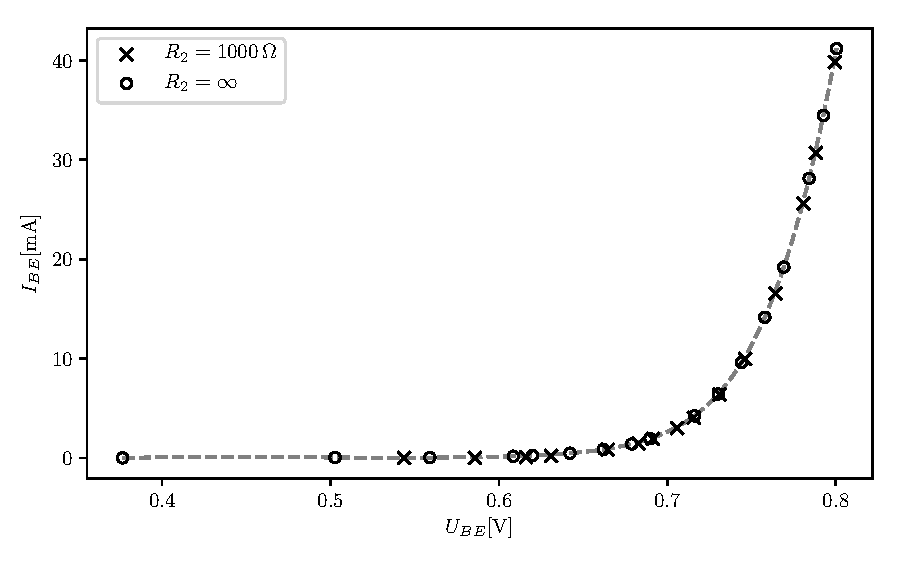
\includegraphics[]{u1}
\caption{Závislost proudu tekoucího bází na napětí mezi bází a emitorem}
\label{fig:u1}
\end{figure}

\begin{figure}[H]
\centering
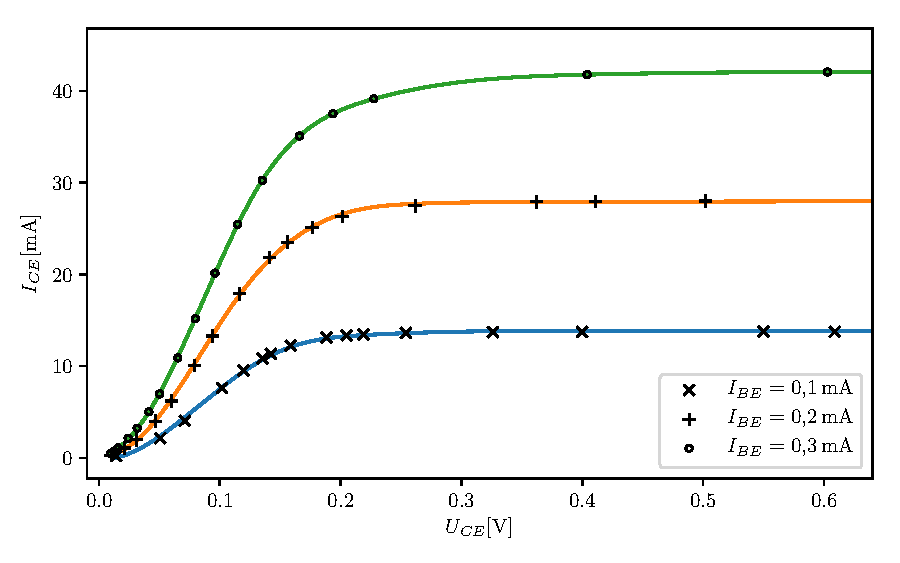
\includegraphics[]{u2}
\caption{Část závislosti proudu tekoucího kolektorem na napětí mezi kolektorem a emitorem}
\label{fig:u2}
\end{figure}

Graf \ref{fig:u3} znázorňuje lineární závislost zesíleného proudu $I_{CE}$ na $I_{BE}$ při třech napětích v kolektorovém obvodu. Tyto závislosti byly proloženy lineárním fitem.

\begin{figure}[H]
\centering
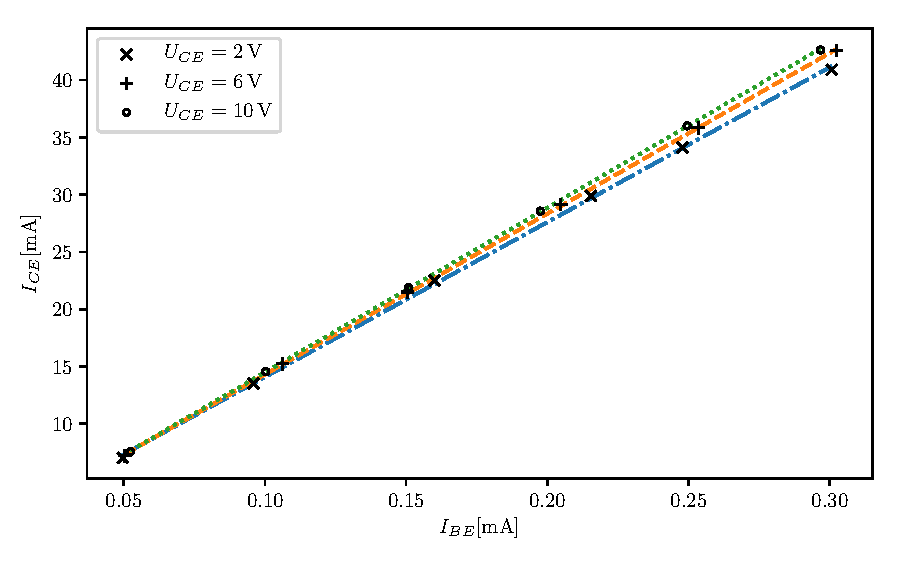
\includegraphics[]{u3}
\caption{Závislost zesíleného proudu $I_{CE}$ na vstupním $I_{BE}$}
\label{fig:u3}
\end{figure}

Směrnice lineárních regresí odpovídají činiteli proudového zesílení 
$$ \beta_{U_{CE} = \SI{2}{V}} = \SI{135.2 \pm 1.3}{}, $$
$$ \beta_{U_{CE} = \SI{6}{V}} = \SI{140.3 \pm 0.6}{}, $$
$$ \beta_{U_{CE} = \SI{10}{V}} = \SI{143.7 \pm 0.4}{}. $$

\end{document}
